Da die Kameraeinstellungen auf die Prüfstation und Prüfbedingungen angepasst werden müssen, sind die Möglichkeiten zur Eliminierung der Streifen im Vorhinein begrenzt.
Die Nachbearbeitung kann über verschiedene Ansätze erfolgen.
Aufgrund der Periodizität und der festen Ausbreitungsrichtung der Streifen bietet es sich an, die Fourier-Analyse anzuwenden.
Man untersucht die Frequenzkomponenten der Streifen und filtert speziell diese aus dem Bild heraus, um sie zu entfernen.
Diese Methode kann allerdings nicht die fehlende Information an den dunklen Streifen wiederherstellen, sondern lediglich eine Bildverbesserung durchführen.
Eine andere Möglichkeit ist das Hinzuziehen von weiteren Bildern.
Da an den Stellen der horizontalen Streifen die Information fehlt, kann man zusätzliche Muster zur Hand nehmen, um die Informationen zusammenzufassen.
Man zieht weitere phasenverschobene Muster hinzu, sodass man eine gerade Anzahl an Phasenverschiebungen hat.
Daraus kann man die Informationen vereinen und eliminiert die horizontalen Streifen.
Im Folgenden werden als Beispiel vier Bilder von Streifenmustern miteinander verknüpft, die je eine versetzte Phase zueinander haben.
Aus den vier aufgenommenen Bildern verknüpft man je zwei Bilder, die eine Phasenverschiebung von $\pi$ zueinander haben, mit der betragsmäßigen Differenz.
Die zwei resultierenden Bilder haben zueinander versetzte Streifen, die aus den Überlappungen entstehen.
Zum Schluss kann man die beiden Bilder so verknüpfen, dass man stets den Bildpunkt mit dem höheren Helligkeitswert nimmt.
Das entspricht der Maximierung.
Analog kann man auch die horizontalen Streifen aus Abbildung \ref{img:minAndMaxLink} eliminieren, in welcher die Typen von Fehlstellen isoliert voneinander betrachtet wurden.
In Abbildung \ref{img:imageTree} werden die einzelnen Schritte dieses Verfahrens veranschaulicht.
Analog lässt sich auch die Verknüpfung von mehr als vier phasenverschobenen Streifenmustern durchführen.

\begin{figure}[H]
	\centering
	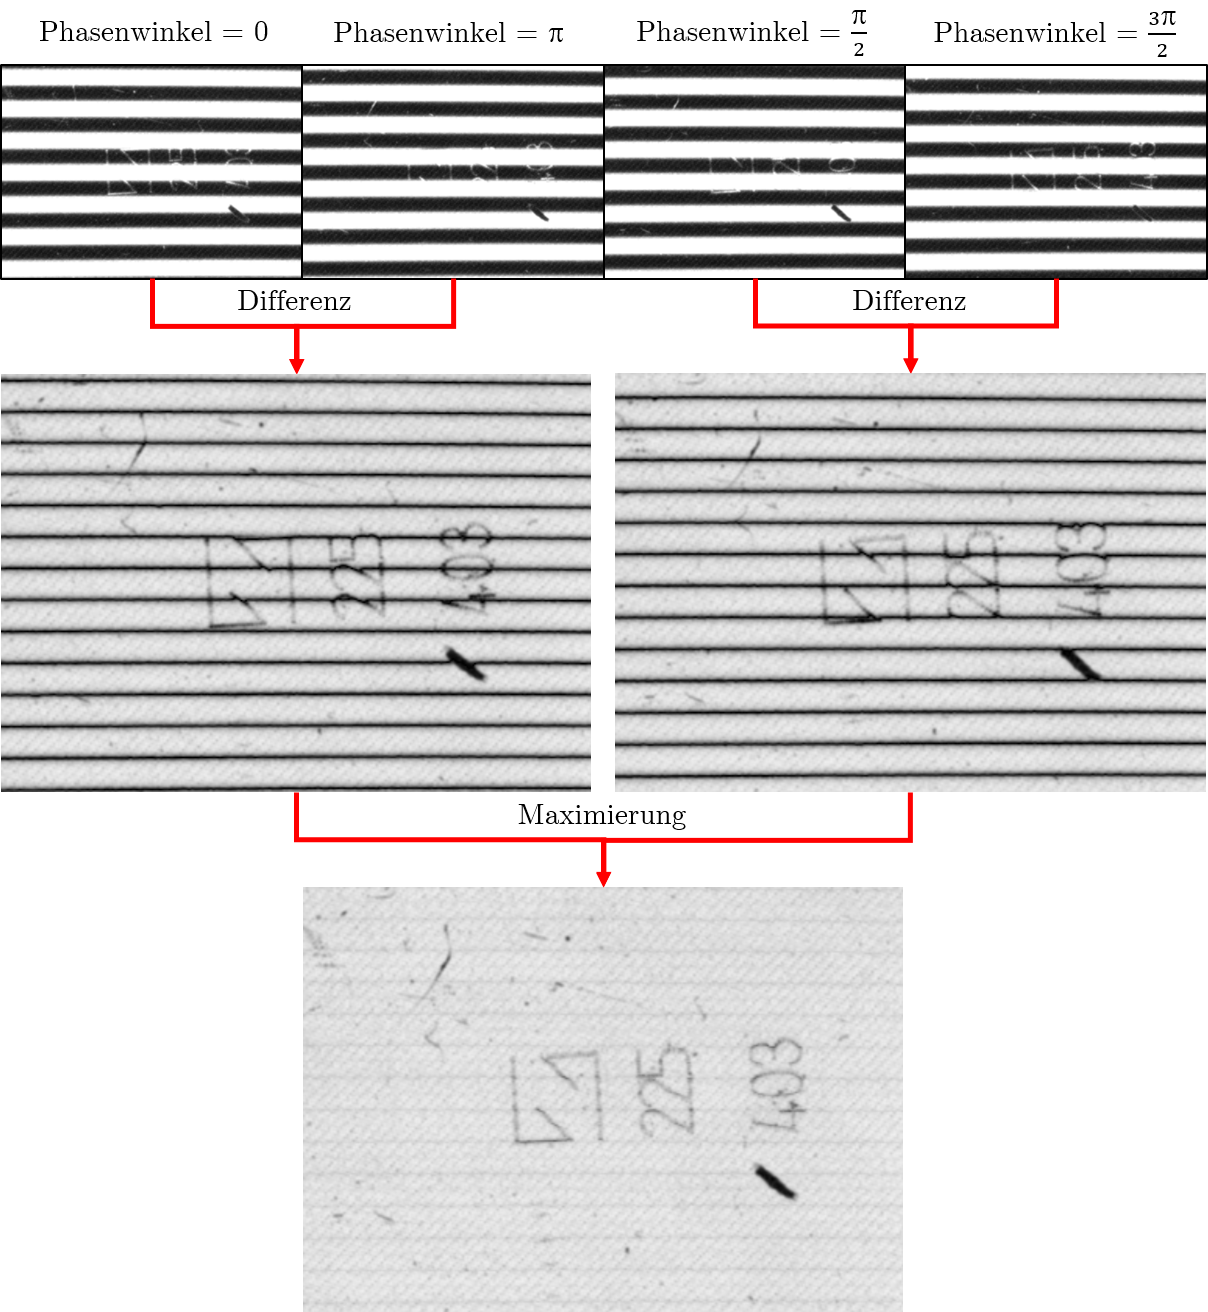
\includegraphics[width=\textwidth]{03_sichtpruefungDurchLichtstreuung/optimierungen/figures/imageTree}
	\caption[Prozess der Hervorhebung von Oberflächendefekten]{Prozess zur Hervorhebung von Oberflächendefekten mit $N_{shift} = 4$.}
	\label{img:imageTree}
\end{figure}